% Created by tikzDevice version 0.10.1 on 2016-04-02 12:23:06
% !TEX encoding = UTF-8 Unicode
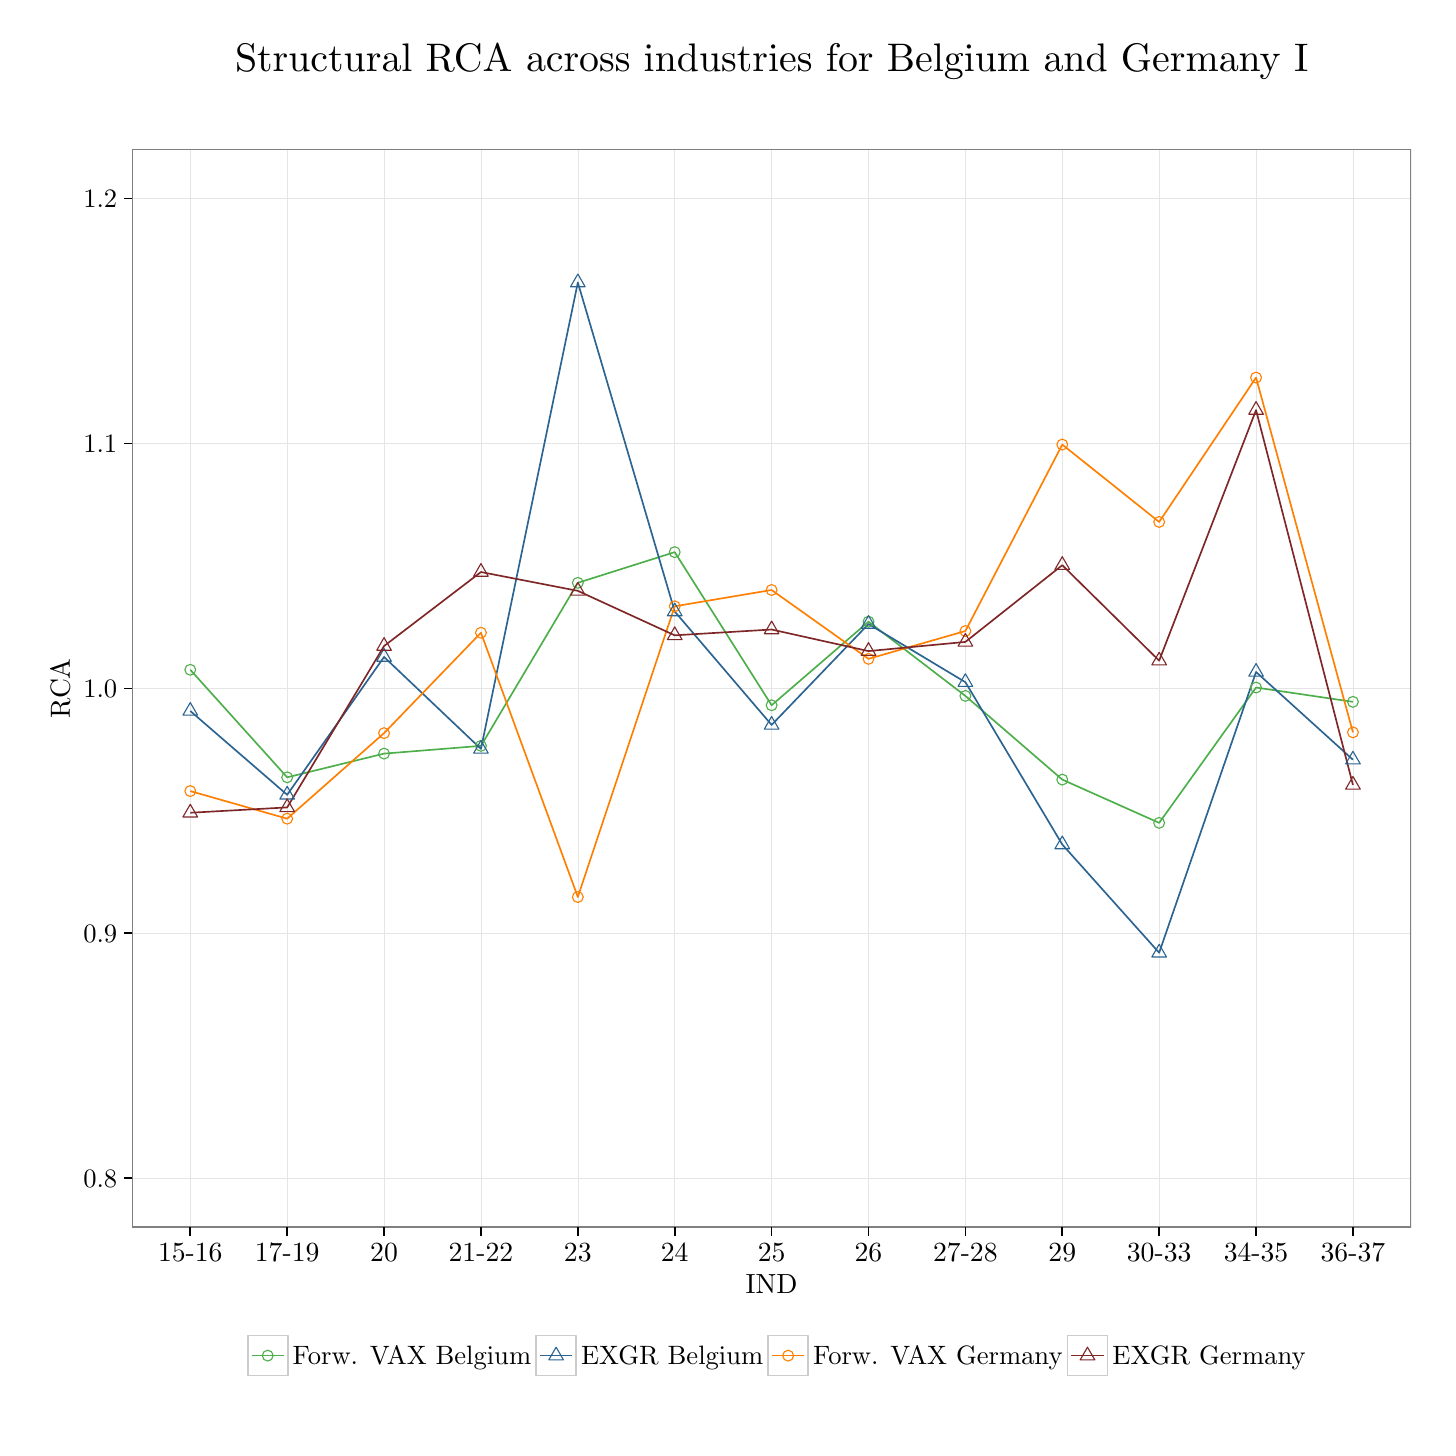
\begin{tikzpicture}[x=1pt,y=1pt]
\definecolor{fillColor}{RGB}{255,255,255}
\path[use as bounding box,fill=fillColor,fill opacity=0.00] (0,0) rectangle (505.89,505.89);
\begin{scope}
\path[clip] (  0.00,  0.00) rectangle (505.89,505.89);
\definecolor{drawColor}{RGB}{255,255,255}
\definecolor{fillColor}{RGB}{255,255,255}

\path[draw=drawColor,line width= 0.6pt,line join=round,line cap=round,fill=fillColor] (  0.00, -0.00) rectangle (505.89,505.89);
\end{scope}
\begin{scope}
\path[clip] ( 37.75, 72.44) rectangle (499.89,461.83);
\definecolor{fillColor}{RGB}{255,255,255}

\path[fill=fillColor] ( 37.75, 72.44) rectangle (499.89,461.83);
\definecolor{drawColor}{gray}{0.90}

\path[draw=drawColor,line width= 0.2pt,line join=round] ( 37.75, 90.14) --
	(499.89, 90.14);

\path[draw=drawColor,line width= 0.2pt,line join=round] ( 37.75,178.64) --
	(499.89,178.64);

\path[draw=drawColor,line width= 0.2pt,line join=round] ( 37.75,267.13) --
	(499.89,267.13);

\path[draw=drawColor,line width= 0.2pt,line join=round] ( 37.75,355.63) --
	(499.89,355.63);

\path[draw=drawColor,line width= 0.2pt,line join=round] ( 37.75,444.13) --
	(499.89,444.13);

\path[draw=drawColor,line width= 0.2pt,line join=round] ( 58.76, 72.44) --
	( 58.76,461.83);

\path[draw=drawColor,line width= 0.2pt,line join=round] ( 93.77, 72.44) --
	( 93.77,461.83);

\path[draw=drawColor,line width= 0.2pt,line join=round] (128.78, 72.44) --
	(128.78,461.83);

\path[draw=drawColor,line width= 0.2pt,line join=round] (163.79, 72.44) --
	(163.79,461.83);

\path[draw=drawColor,line width= 0.2pt,line join=round] (198.80, 72.44) --
	(198.80,461.83);

\path[draw=drawColor,line width= 0.2pt,line join=round] (233.81, 72.44) --
	(233.81,461.83);

\path[draw=drawColor,line width= 0.2pt,line join=round] (268.82, 72.44) --
	(268.82,461.83);

\path[draw=drawColor,line width= 0.2pt,line join=round] (303.83, 72.44) --
	(303.83,461.83);

\path[draw=drawColor,line width= 0.2pt,line join=round] (338.84, 72.44) --
	(338.84,461.83);

\path[draw=drawColor,line width= 0.2pt,line join=round] (373.85, 72.44) --
	(373.85,461.83);

\path[draw=drawColor,line width= 0.2pt,line join=round] (408.86, 72.44) --
	(408.86,461.83);

\path[draw=drawColor,line width= 0.2pt,line join=round] (443.87, 72.44) --
	(443.87,461.83);

\path[draw=drawColor,line width= 0.2pt,line join=round] (478.88, 72.44) --
	(478.88,461.83);
\definecolor{drawColor}{RGB}{77,175,74}

\path[draw=drawColor,line width= 0.6pt,line join=round] ( 58.76,273.86) --
	( 93.77,235.00) --
	(128.78,243.57) --
	(163.79,246.37) --
	(198.80,305.28) --
	(233.81,316.37) --
	(268.82,261.04) --
	(303.83,291.25) --
	(338.84,264.42) --
	(373.85,234.18) --
	(408.86,218.54) --
	(443.87,267.44) --
	(478.88,262.28);
\definecolor{drawColor}{RGB}{43,99,145}

\path[draw=drawColor,line width= 0.6pt,line join=round] ( 58.76,258.97) --
	( 93.77,228.68) --
	(128.78,278.49) --
	(163.79,245.26) --
	(198.80,413.81) --
	(233.81,294.92) --
	(268.82,253.93) --
	(303.83,290.39) --
	(338.84,269.38) --
	(373.85,210.73) --
	(408.86,171.61) --
	(443.87,273.07) --
	(478.88,241.36);
\definecolor{drawColor}{RGB}{255,127,0}

\path[draw=drawColor,line width= 0.6pt,line join=round] ( 58.76,230.03) --
	( 93.77,220.06) --
	(128.78,250.97) --
	(163.79,287.25) --
	(198.80,191.75) --
	(233.81,296.80) --
	(268.82,302.69) --
	(303.83,277.81) --
	(338.84,287.87) --
	(373.85,355.24) --
	(408.86,327.28) --
	(443.87,379.45) --
	(478.88,251.25);
\definecolor{drawColor}{RGB}{127,38,39}

\path[draw=drawColor,line width= 0.6pt,line join=round] ( 58.76,222.20) --
	( 93.77,224.13) --
	(128.78,282.44) --
	(163.79,309.18) --
	(198.80,302.38) --
	(233.81,286.31) --
	(268.82,288.41) --
	(303.83,280.61) --
	(338.84,283.93) --
	(373.85,311.66) --
	(408.86,277.15) --
	(443.87,367.71) --
	(478.88,232.26);
\definecolor{drawColor}{RGB}{77,175,74}

\path[draw=drawColor,line width= 0.4pt,line join=round,line cap=round] ( 58.76,273.86) circle (  1.96);

\path[draw=drawColor,line width= 0.4pt,line join=round,line cap=round] ( 93.77,235.00) circle (  1.96);

\path[draw=drawColor,line width= 0.4pt,line join=round,line cap=round] (128.78,243.57) circle (  1.96);

\path[draw=drawColor,line width= 0.4pt,line join=round,line cap=round] (163.79,246.37) circle (  1.96);

\path[draw=drawColor,line width= 0.4pt,line join=round,line cap=round] (198.80,305.28) circle (  1.96);

\path[draw=drawColor,line width= 0.4pt,line join=round,line cap=round] (233.81,316.37) circle (  1.96);

\path[draw=drawColor,line width= 0.4pt,line join=round,line cap=round] (268.82,261.04) circle (  1.96);

\path[draw=drawColor,line width= 0.4pt,line join=round,line cap=round] (303.83,291.25) circle (  1.96);

\path[draw=drawColor,line width= 0.4pt,line join=round,line cap=round] (338.84,264.42) circle (  1.96);

\path[draw=drawColor,line width= 0.4pt,line join=round,line cap=round] (373.85,234.18) circle (  1.96);

\path[draw=drawColor,line width= 0.4pt,line join=round,line cap=round] (408.86,218.54) circle (  1.96);

\path[draw=drawColor,line width= 0.4pt,line join=round,line cap=round] (443.87,267.44) circle (  1.96);

\path[draw=drawColor,line width= 0.4pt,line join=round,line cap=round] (478.88,262.28) circle (  1.96);
\definecolor{drawColor}{RGB}{255,127,0}

\path[draw=drawColor,line width= 0.4pt,line join=round,line cap=round] ( 58.76,230.03) circle (  1.96);

\path[draw=drawColor,line width= 0.4pt,line join=round,line cap=round] ( 93.77,220.06) circle (  1.96);

\path[draw=drawColor,line width= 0.4pt,line join=round,line cap=round] (128.78,250.97) circle (  1.96);

\path[draw=drawColor,line width= 0.4pt,line join=round,line cap=round] (163.79,287.25) circle (  1.96);

\path[draw=drawColor,line width= 0.4pt,line join=round,line cap=round] (198.80,191.75) circle (  1.96);

\path[draw=drawColor,line width= 0.4pt,line join=round,line cap=round] (233.81,296.80) circle (  1.96);

\path[draw=drawColor,line width= 0.4pt,line join=round,line cap=round] (268.82,302.69) circle (  1.96);

\path[draw=drawColor,line width= 0.4pt,line join=round,line cap=round] (303.83,277.81) circle (  1.96);

\path[draw=drawColor,line width= 0.4pt,line join=round,line cap=round] (338.84,287.87) circle (  1.96);

\path[draw=drawColor,line width= 0.4pt,line join=round,line cap=round] (373.85,355.24) circle (  1.96);

\path[draw=drawColor,line width= 0.4pt,line join=round,line cap=round] (408.86,327.28) circle (  1.96);

\path[draw=drawColor,line width= 0.4pt,line join=round,line cap=round] (443.87,379.45) circle (  1.96);

\path[draw=drawColor,line width= 0.4pt,line join=round,line cap=round] (478.88,251.25) circle (  1.96);
\definecolor{drawColor}{RGB}{43,99,145}

\path[draw=drawColor,line width= 0.4pt,line join=round,line cap=round] ( 58.76,262.02) --
	( 61.40,257.45) --
	( 56.11,257.45) --
	( 58.76,262.02);

\path[draw=drawColor,line width= 0.4pt,line join=round,line cap=round] ( 93.77,231.74) --
	( 96.41,227.16) --
	( 91.13,227.16) --
	( 93.77,231.74);

\path[draw=drawColor,line width= 0.4pt,line join=round,line cap=round] (128.78,281.54) --
	(131.42,276.96) --
	(126.14,276.96) --
	(128.78,281.54);

\path[draw=drawColor,line width= 0.4pt,line join=round,line cap=round] (163.79,248.31) --
	(166.43,243.74) --
	(161.15,243.74) --
	(163.79,248.31);

\path[draw=drawColor,line width= 0.4pt,line join=round,line cap=round] (198.80,416.86) --
	(201.44,412.28) --
	(196.16,412.28) --
	(198.80,416.86);

\path[draw=drawColor,line width= 0.4pt,line join=round,line cap=round] (233.81,297.97) --
	(236.45,293.39) --
	(231.17,293.39) --
	(233.81,297.97);

\path[draw=drawColor,line width= 0.4pt,line join=round,line cap=round] (268.82,256.99) --
	(271.46,252.41) --
	(266.18,252.41) --
	(268.82,256.99);

\path[draw=drawColor,line width= 0.4pt,line join=round,line cap=round] (303.83,293.44) --
	(306.47,288.87) --
	(301.19,288.87) --
	(303.83,293.44);

\path[draw=drawColor,line width= 0.4pt,line join=round,line cap=round] (338.84,272.43) --
	(341.48,267.86) --
	(336.20,267.86) --
	(338.84,272.43);

\path[draw=drawColor,line width= 0.4pt,line join=round,line cap=round] (373.85,213.79) --
	(376.49,209.21) --
	(371.21,209.21) --
	(373.85,213.79);

\path[draw=drawColor,line width= 0.4pt,line join=round,line cap=round] (408.86,174.66) --
	(411.51,170.09) --
	(406.22,170.09) --
	(408.86,174.66);

\path[draw=drawColor,line width= 0.4pt,line join=round,line cap=round] (443.87,276.12) --
	(446.52,271.55) --
	(441.23,271.55) --
	(443.87,276.12);

\path[draw=drawColor,line width= 0.4pt,line join=round,line cap=round] (478.88,244.41) --
	(481.53,239.84) --
	(476.24,239.84) --
	(478.88,244.41);
\definecolor{drawColor}{RGB}{127,38,39}

\path[draw=drawColor,line width= 0.4pt,line join=round,line cap=round] ( 58.76,225.25) --
	( 61.40,220.68) --
	( 56.11,220.68) --
	( 58.76,225.25);

\path[draw=drawColor,line width= 0.4pt,line join=round,line cap=round] ( 93.77,227.18) --
	( 96.41,222.61) --
	( 91.13,222.61) --
	( 93.77,227.18);

\path[draw=drawColor,line width= 0.4pt,line join=round,line cap=round] (128.78,285.49) --
	(131.42,280.92) --
	(126.14,280.92) --
	(128.78,285.49);

\path[draw=drawColor,line width= 0.4pt,line join=round,line cap=round] (163.79,312.23) --
	(166.43,307.65) --
	(161.15,307.65) --
	(163.79,312.23);

\path[draw=drawColor,line width= 0.4pt,line join=round,line cap=round] (198.80,305.43) --
	(201.44,300.86) --
	(196.16,300.86) --
	(198.80,305.43);

\path[draw=drawColor,line width= 0.4pt,line join=round,line cap=round] (233.81,289.36) --
	(236.45,284.78) --
	(231.17,284.78) --
	(233.81,289.36);

\path[draw=drawColor,line width= 0.4pt,line join=round,line cap=round] (268.82,291.46) --
	(271.46,286.89) --
	(266.18,286.89) --
	(268.82,291.46);

\path[draw=drawColor,line width= 0.4pt,line join=round,line cap=round] (303.83,283.66) --
	(306.47,279.09) --
	(301.19,279.09) --
	(303.83,283.66);

\path[draw=drawColor,line width= 0.4pt,line join=round,line cap=round] (338.84,286.98) --
	(341.48,282.40) --
	(336.20,282.40) --
	(338.84,286.98);

\path[draw=drawColor,line width= 0.4pt,line join=round,line cap=round] (373.85,314.72) --
	(376.49,310.14) --
	(371.21,310.14) --
	(373.85,314.72);

\path[draw=drawColor,line width= 0.4pt,line join=round,line cap=round] (408.86,280.20) --
	(411.51,275.63) --
	(406.22,275.63) --
	(408.86,280.20);

\path[draw=drawColor,line width= 0.4pt,line join=round,line cap=round] (443.87,370.76) --
	(446.52,366.19) --
	(441.23,366.19) --
	(443.87,370.76);

\path[draw=drawColor,line width= 0.4pt,line join=round,line cap=round] (478.88,235.31) --
	(481.53,230.73) --
	(476.24,230.73) --
	(478.88,235.31);
\definecolor{drawColor}{gray}{0.50}

\path[draw=drawColor,line width= 0.6pt,line join=round,line cap=round] ( 37.75, 72.44) rectangle (499.89,461.83);
\end{scope}
\begin{scope}
\path[clip] (  0.00,  0.00) rectangle (505.89,505.89);
\definecolor{drawColor}{RGB}{0,0,0}

\node[text=drawColor,anchor=base east,inner sep=0pt, outer sep=0pt, scale=  0.96] at ( 32.35, 86.83) {0.8};

\node[text=drawColor,anchor=base east,inner sep=0pt, outer sep=0pt, scale=  0.96] at ( 32.35,175.33) {0.9};

\node[text=drawColor,anchor=base east,inner sep=0pt, outer sep=0pt, scale=  0.96] at ( 32.35,263.83) {1.0};

\node[text=drawColor,anchor=base east,inner sep=0pt, outer sep=0pt, scale=  0.96] at ( 32.35,352.33) {1.1};

\node[text=drawColor,anchor=base east,inner sep=0pt, outer sep=0pt, scale=  0.96] at ( 32.35,440.83) {1.2};
\end{scope}
\begin{scope}
\path[clip] (  0.00,  0.00) rectangle (505.89,505.89);
\definecolor{drawColor}{RGB}{0,0,0}

\path[draw=drawColor,line width= 0.6pt,line join=round] ( 34.75, 90.14) --
	( 37.75, 90.14);

\path[draw=drawColor,line width= 0.6pt,line join=round] ( 34.75,178.64) --
	( 37.75,178.64);

\path[draw=drawColor,line width= 0.6pt,line join=round] ( 34.75,267.13) --
	( 37.75,267.13);

\path[draw=drawColor,line width= 0.6pt,line join=round] ( 34.75,355.63) --
	( 37.75,355.63);

\path[draw=drawColor,line width= 0.6pt,line join=round] ( 34.75,444.13) --
	( 37.75,444.13);
\end{scope}
\begin{scope}
\path[clip] (  0.00,  0.00) rectangle (505.89,505.89);
\definecolor{drawColor}{RGB}{0,0,0}

\path[draw=drawColor,line width= 0.6pt,line join=round] ( 58.76, 69.44) --
	( 58.76, 72.44);

\path[draw=drawColor,line width= 0.6pt,line join=round] ( 93.77, 69.44) --
	( 93.77, 72.44);

\path[draw=drawColor,line width= 0.6pt,line join=round] (128.78, 69.44) --
	(128.78, 72.44);

\path[draw=drawColor,line width= 0.6pt,line join=round] (163.79, 69.44) --
	(163.79, 72.44);

\path[draw=drawColor,line width= 0.6pt,line join=round] (198.80, 69.44) --
	(198.80, 72.44);

\path[draw=drawColor,line width= 0.6pt,line join=round] (233.81, 69.44) --
	(233.81, 72.44);

\path[draw=drawColor,line width= 0.6pt,line join=round] (268.82, 69.44) --
	(268.82, 72.44);

\path[draw=drawColor,line width= 0.6pt,line join=round] (303.83, 69.44) --
	(303.83, 72.44);

\path[draw=drawColor,line width= 0.6pt,line join=round] (338.84, 69.44) --
	(338.84, 72.44);

\path[draw=drawColor,line width= 0.6pt,line join=round] (373.85, 69.44) --
	(373.85, 72.44);

\path[draw=drawColor,line width= 0.6pt,line join=round] (408.86, 69.44) --
	(408.86, 72.44);

\path[draw=drawColor,line width= 0.6pt,line join=round] (443.87, 69.44) --
	(443.87, 72.44);

\path[draw=drawColor,line width= 0.6pt,line join=round] (478.88, 69.44) --
	(478.88, 72.44);
\end{scope}
\begin{scope}
\path[clip] (  0.00,  0.00) rectangle (505.89,505.89);
\definecolor{drawColor}{RGB}{0,0,0}

\node[text=drawColor,anchor=base,inner sep=0pt, outer sep=0pt, scale=  1.00] at ( 58.76, 60.15) {15-16};

\node[text=drawColor,anchor=base,inner sep=0pt, outer sep=0pt, scale=  1.00] at ( 93.77, 60.15) {17-19};

\node[text=drawColor,anchor=base,inner sep=0pt, outer sep=0pt, scale=  1.00] at (128.78, 60.15) {20};

\node[text=drawColor,anchor=base,inner sep=0pt, outer sep=0pt, scale=  1.00] at (163.79, 60.15) {21-22};

\node[text=drawColor,anchor=base,inner sep=0pt, outer sep=0pt, scale=  1.00] at (198.80, 60.15) {23};

\node[text=drawColor,anchor=base,inner sep=0pt, outer sep=0pt, scale=  1.00] at (233.81, 60.15) {24};

\node[text=drawColor,anchor=base,inner sep=0pt, outer sep=0pt, scale=  1.00] at (268.82, 60.15) {25};

\node[text=drawColor,anchor=base,inner sep=0pt, outer sep=0pt, scale=  1.00] at (303.83, 60.15) {26};

\node[text=drawColor,anchor=base,inner sep=0pt, outer sep=0pt, scale=  1.00] at (338.84, 60.15) {27-28};

\node[text=drawColor,anchor=base,inner sep=0pt, outer sep=0pt, scale=  1.00] at (373.85, 60.15) {29};

\node[text=drawColor,anchor=base,inner sep=0pt, outer sep=0pt, scale=  1.00] at (408.86, 60.15) {30-33};

\node[text=drawColor,anchor=base,inner sep=0pt, outer sep=0pt, scale=  1.00] at (443.87, 60.15) {34-35};

\node[text=drawColor,anchor=base,inner sep=0pt, outer sep=0pt, scale=  1.00] at (478.88, 60.15) {36-37};
\end{scope}
\begin{scope}
\path[clip] (  0.00,  0.00) rectangle (505.89,505.89);
\definecolor{drawColor}{RGB}{0,0,0}

\node[text=drawColor,anchor=base,inner sep=0pt, outer sep=0pt, scale=  1.00] at (268.82, 48.46) {IND};
\end{scope}
\begin{scope}
\path[clip] (  0.00,  0.00) rectangle (505.89,505.89);
\definecolor{drawColor}{RGB}{0,0,0}

\node[text=drawColor,rotate= 90.00,anchor=base,inner sep=0pt, outer sep=0pt, scale=  1.00] at ( 15.29,267.13) {RCA};
\end{scope}
\begin{scope}
\path[clip] (  0.00,  0.00) rectangle (505.89,505.89);
\definecolor{fillColor}{RGB}{255,255,255}

\path[fill=fillColor] ( 71.63, 14.54) rectangle (466.01, 37.53);
\end{scope}
\begin{scope}
\path[clip] (  0.00,  0.00) rectangle (505.89,505.89);
\definecolor{drawColor}{gray}{0.80}
\definecolor{fillColor}{RGB}{255,255,255}

\path[draw=drawColor,line width= 0.6pt,line join=round,line cap=round,fill=fillColor] ( 79.51, 18.80) rectangle ( 93.97, 33.26);
\end{scope}
\begin{scope}
\path[clip] (  0.00,  0.00) rectangle (505.89,505.89);
\definecolor{drawColor}{RGB}{77,175,74}

\path[draw=drawColor,line width= 0.6pt,line join=round] ( 80.96, 26.03) -- ( 92.52, 26.03);
\end{scope}
\begin{scope}
\path[clip] (  0.00,  0.00) rectangle (505.89,505.89);
\definecolor{drawColor}{RGB}{77,175,74}

\path[draw=drawColor,line width= 0.4pt,line join=round,line cap=round] ( 86.74, 26.03) circle (  1.96);
\end{scope}
\begin{scope}
\path[clip] (  0.00,  0.00) rectangle (505.89,505.89);
\definecolor{drawColor}{gray}{0.80}
\definecolor{fillColor}{RGB}{255,255,255}

\path[draw=drawColor,line width= 0.6pt,line join=round,line cap=round,fill=fillColor] (183.72, 18.80) rectangle (198.17, 33.26);
\end{scope}
\begin{scope}
\path[clip] (  0.00,  0.00) rectangle (505.89,505.89);
\definecolor{drawColor}{RGB}{43,99,145}

\path[draw=drawColor,line width= 0.6pt,line join=round] (185.17, 26.03) -- (196.73, 26.03);
\end{scope}
\begin{scope}
\path[clip] (  0.00,  0.00) rectangle (505.89,505.89);
\definecolor{drawColor}{RGB}{43,99,145}

\path[draw=drawColor,line width= 0.4pt,line join=round,line cap=round] (190.95, 29.08) --
	(193.59, 24.51) --
	(188.30, 24.51) --
	(190.95, 29.08);
\end{scope}
\begin{scope}
\path[clip] (  0.00,  0.00) rectangle (505.89,505.89);
\definecolor{drawColor}{gray}{0.80}
\definecolor{fillColor}{RGB}{255,255,255}

\path[draw=drawColor,line width= 0.6pt,line join=round,line cap=round,fill=fillColor] (267.57, 18.80) rectangle (282.03, 33.26);
\end{scope}
\begin{scope}
\path[clip] (  0.00,  0.00) rectangle (505.89,505.89);
\definecolor{drawColor}{RGB}{255,127,0}

\path[draw=drawColor,line width= 0.6pt,line join=round] (269.02, 26.03) -- (280.58, 26.03);
\end{scope}
\begin{scope}
\path[clip] (  0.00,  0.00) rectangle (505.89,505.89);
\definecolor{drawColor}{RGB}{255,127,0}

\path[draw=drawColor,line width= 0.4pt,line join=round,line cap=round] (274.80, 26.03) circle (  1.96);
\end{scope}
\begin{scope}
\path[clip] (  0.00,  0.00) rectangle (505.89,505.89);
\definecolor{drawColor}{gray}{0.80}
\definecolor{fillColor}{RGB}{255,255,255}

\path[draw=drawColor,line width= 0.6pt,line join=round,line cap=round,fill=fillColor] (375.74, 18.80) rectangle (390.19, 33.26);
\end{scope}
\begin{scope}
\path[clip] (  0.00,  0.00) rectangle (505.89,505.89);
\definecolor{drawColor}{RGB}{127,38,39}

\path[draw=drawColor,line width= 0.6pt,line join=round] (377.18, 26.03) -- (388.75, 26.03);
\end{scope}
\begin{scope}
\path[clip] (  0.00,  0.00) rectangle (505.89,505.89);
\definecolor{drawColor}{RGB}{127,38,39}

\path[draw=drawColor,line width= 0.4pt,line join=round,line cap=round] (382.96, 29.08) --
	(385.61, 24.51) --
	(380.32, 24.51) --
	(382.96, 29.08);
\end{scope}
\begin{scope}
\path[clip] (  0.00,  0.00) rectangle (505.89,505.89);
\definecolor{drawColor}{RGB}{0,0,0}

\node[text=drawColor,anchor=base west,inner sep=0pt, outer sep=0pt, scale=  0.96] at ( 95.77, 22.72) {Forw. VAX Belgium};
\end{scope}
\begin{scope}
\path[clip] (  0.00,  0.00) rectangle (505.89,505.89);
\definecolor{drawColor}{RGB}{0,0,0}

\node[text=drawColor,anchor=base west,inner sep=0pt, outer sep=0pt, scale=  0.96] at (199.98, 22.72) {EXGR Belgium};
\end{scope}
\begin{scope}
\path[clip] (  0.00,  0.00) rectangle (505.89,505.89);
\definecolor{drawColor}{RGB}{0,0,0}

\node[text=drawColor,anchor=base west,inner sep=0pt, outer sep=0pt, scale=  0.96] at (283.83, 22.72) {Forw. VAX Germany};
\end{scope}
\begin{scope}
\path[clip] (  0.00,  0.00) rectangle (505.89,505.89);
\definecolor{drawColor}{RGB}{0,0,0}

\node[text=drawColor,anchor=base west,inner sep=0pt, outer sep=0pt, scale=  0.96] at (392.00, 22.72) {EXGR Germany};
\end{scope}
\begin{scope}
\path[clip] (  0.00,  0.00) rectangle (505.89,505.89);
\definecolor{drawColor}{RGB}{0,0,0}

\node[text=drawColor,anchor=base west,inner sep=0pt, outer sep=0pt, scale=  1.44] at ( 74.94,489.97) {Structural RCA across industries for Belgium and Germany I};
\end{scope}
\end{tikzpicture}
